\documentclass[11pt,a4paper]{article}
\usepackage[margin=1in]{geometry}
\usepackage{times}
\usepackage[T1]{fontenc}
\usepackage[utf8]{inputenc}
\usepackage{amsmath,amssymb}
\usepackage{booktabs}
\usepackage{graphicx}
\usepackage{subcaption}
\usepackage{multicol}
\usepackage{parskip}
\usepackage{linguex}
\usepackage[numbers,sort&compress]{natbib}
\usepackage[hidelinks]{hyperref}
\usepackage{stmaryrd}
\usepackage[font=small]{caption}

\pagestyle{empty}
\setlength{\abovedisplayskip}{5pt}
\setlength{\belowdisplayskip}{5pt}
\setlength{\parskip}{3pt}

\begin{document}

\noindent\textbf{\large From Controversy to Consensus: Modelling Community-Sensitive Common Ground \\ Management in German Discourse Markers}

\smallskip

\noindent This study investigates three German discourse markers, which we label \emph{consensus markers}---\textit{soviel ich wei\ss} (`as far as I know'), \textit{ja} (roughly `as you know'), and \textit{bekanntlich} (`as is well known').
Intuitively, these markers differ in how they allow a speaker to present $p$ as settled in a given common ground.
We ask whether this intuition can be formalized in a probabilistic pragmatic model that infers marker-specific felicity thresholds from production choices and uses them to predict marker choice and listener interpretation as controversy, community, and goal vary.
\ex. \textit{Impfungen sind (soviel ich wei\ss / ja / bekanntlich) sicher und wirksam; deshalb solltest du dich impfen lassen.}\\
`Vaccinations are, as far as I know / as you know / as is well known, safe and effective; therefore you should get vaccinated.'
\z.
With \textit{soviel ich wei\ss}, the speaker restricts $p$ to their own epistemic state; \textit{ja} presents $p$ as shared with the addressee; and \textit{bekanntlich} presents $p$ as more broadly publicly accessible knowledge.
The felicity of each marker therefore depends on several dimensions at once.
First, the status of $p$ is community-relative: the safety and efficacy of vaccination may be treated as settled in a medical-expert community, but remain contested in a divided public setting.
Second, the speaker's goal matters.
A political group promoting vaccination, for instance, may have an interest in presenting $p$ as already settled, because doing so strengthens the move from $p$ to the recommendation $q$.
Third, propositions differ in their baseline degree of controversy, independently of the immediate discourse context.
Thus, by selecting a particular consensus marker, the speaker can present p as more or less settled and thereby guide the addressee toward accepting q as a recommendation grounded in shared assumptions.

We use the label \emph{consensus markers} functionally: the three expressions differ in syntactic category and lexical meaning, but all bear on how $p$ is managed in the common ground.
Previous work on German discourse particles treats \textit{ja} as contributing non-truth-conditional, use-conditional meaning \citep{gutzmann2015use,grosz2021discourse}.
Its common-ground effect has been characterized as marking $p$ as \textsc{known} \citep{thurmair1989modalpartikeln}, speaker-assumed common knowledge \citep{karagjosova2004meaning}, uncontroversial \citep{jacobs_semantics_1991,zimmermann2011discourse,waltereit2001modal}, settled in the common ground \citep{repp2013common}, or available for manipulative use in convincing an interlocutor \citep{doring2016modal}.
Recent experimental work further links \textit{ja} to causal discourse contexts \citep{seemann2025}, motivating the running setup in (1), where $p$ serves as the premise for the downstream recommendation $q$.
What remains missing is a formal account of marker felicity that integrates community-relative consensus around $p$ with the speaker’s communicative goal in presenting $p$ as support for $q$.

Building on these insights, we propose a utility-based, noisy-threshold model within probabilistic pragmatics \citep{goodman2016pragmatic, franke2016probabilistic, degen2023rational}.
The central modelling contribution is to infer these felicity thresholds from production data and use posterior predictions for item selection of listener's tasks to connect production and interpretation.
Marker choice is modelled as a decision about whether $p$ can be presented as a sufficiently settled premise for $q$.
This brings together the propositional controversy of $p$, the pragmatic status of $p$ in a relevant epistemic community, and the speaker's goal in using $p$ to support $q$.
Empirically, we implement this link in a three-step pipeline (Fig.~\ref{fig:overview}): norming estimates baseline propositional controversy, production estimates how pragmatic controversy and goal strength shape marker choice, and comprehension tests whether listeners recover speaker goals and adoption consequences from the chosen marker.
The empirical findings are graded in both production and interpretation: lower controversy and higher goal strength favour stricter thresholds, and the corresponding markers lead listeners to infer stronger speaker goals.
For adoption, weakly supported felicity conditions can make the speaker's attempt to present $p$ as settled visible, leading listeners to discount the recommendation, in line with pragmatic reactance \citep{Brehm1966-BREATO-2}.
Fitted to the production data, the model estimates partially overlapping felicity thresholds for \textit{ja} and \textit{bekanntlich} from speakers' choices across contexts.
Taken together, the results show that consensus markers constrain how $p$ can be presented as a shared premise for $q$, with speaker choice and listener inference shaped by the relevant epistemic community and the speaker's goal.

\newpage
\textbf{Model.}\footnote{Implemented in Stan; MCMC inference used the No-U-Turn Sampler \citep{carpenter2017stan,hoffman2014nuts}.}
Perceived controversy combines propositional and pragmatic components, $pc = pc_{\text{prop}} \cdot pc_{\text{prag}}$, and enters a utility $U(pc, g) = -w_{pc} \cdot pc + w_g \cdot g - w_{int} \cdot pc \cdot g$, where $g$ is the speaker's goal strength.
Low controversy and high goal strength jointly favour stricter thresholds, while $w_{int}$ captures the additional cost of invoking consensus under high controversy.
Each marker $u_i$ is associated with a noisy interval $[\theta_i, \theta_{i+1})$ on the utility scale, so relative position and overlap are inferred from choices.
A marker is selected when $U$ falls within its interval, $P(u_i \mid pc, g) \propto \sigma(\lambda(U - \theta_i)) \cdot \sigma(-\lambda(U - \theta_{i+1}))$, and a pragmatic listener inverts this model to infer $pc$ and $g$.

\textbf{Empirical evidence.}\footnote{Reported coefficients and one-sided probabilities come from Bayesian regression models; hypotheses were evaluated using posterior predictions.}
The experiments implement the pipeline summarized above (Fig.~\ref{fig:overview}).
In production (Fig.~\ref{fig:production}), $g$ favours stricter-threshold markers ($0.28$, $P(>0) = 1$) and $pc_{\text{prag}}$ disfavours them ($-0.17$, $P(<0) = 0.98$); the goal effect shrinks under high controversy (interaction: $-0.22$, $P(<0) = 0.97$), as predicted by the $w_{int}$ cost term.
In comprehension (Fig.~\ref{fig:comprehension}), both \textit{ja} ($0.49$, $P(>0) = 1$) and \textit{bekanntlich} ($0.46$, $P(>0) = 1$) increase inferred $g$; for adoption, \textit{ja} shows a credible positive effect ($0.42$, $P(>0) = 0.99$), and \textit{bekanntlich} shows a weaker one ($0.17$, $P(>0) = 0.90$).
This dissociation is compatible with pragmatic reactance \citep{Brehm1966-BREATO-2}: listeners infer the speaker's goal from marker choice, then discount weakly supported consensus marking as argumentative pressure.
Our production-trained noisy-threshold model captures these patterns within a single framework.

% ============================================================
% PAGE 2: FIGURES
% ============================================================
\begin{figure}[h!]
  \centering
  \begin{subfigure}[b]{0.49\textwidth}
    \centering
    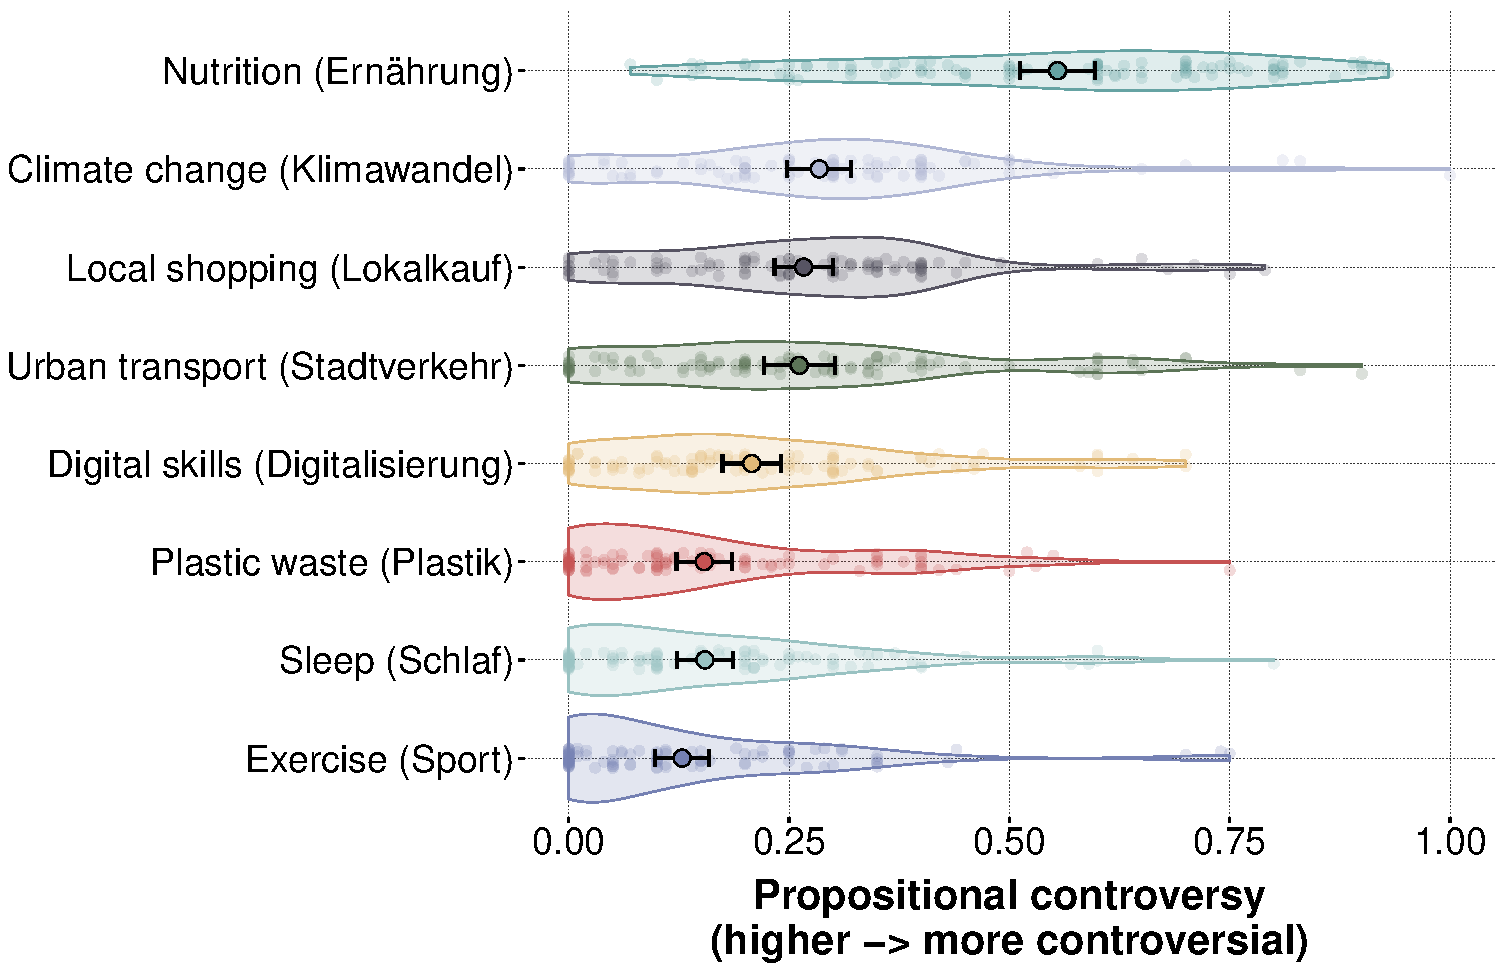
\includegraphics[width=\textwidth]{../../analysis/norming_exp/plots/norming_topic_means.pdf}
    \caption{Norming experiment ($N\!=\!102$): topics differ in baseline propositional controversy.
    German originals in parentheses.}\label{fig:norming}
  \end{subfigure}\hfill
  \begin{subfigure}[b]{0.49\textwidth}
    \centering
    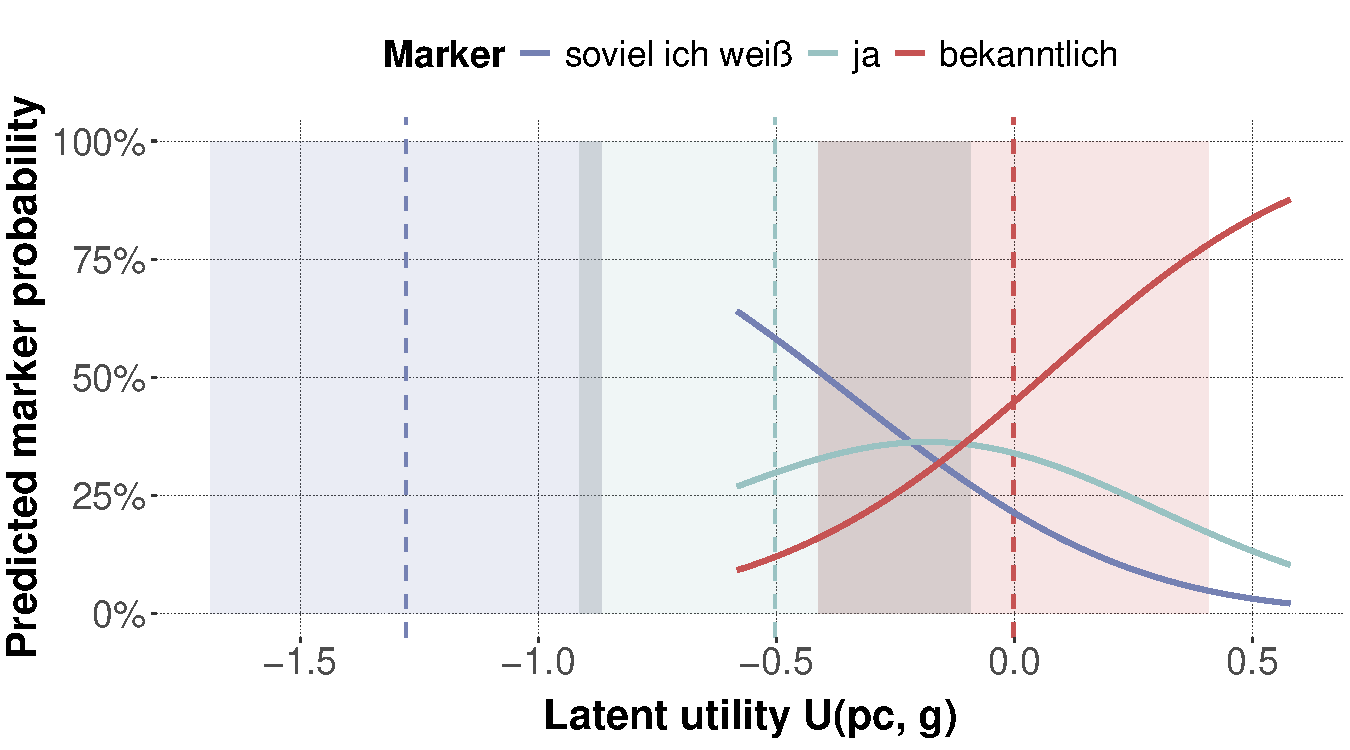
\includegraphics[width=\textwidth]{../../analysis/production_exp/plots/fig11_rsa_soft_thresholds.pdf}
    \caption{Estimated noisy thresholds along the latent utility axis.
    Dashed lines: mean thresholds; shaded bands: overlap.
    The relevant variation falls mainly between \textit{ja} (roughly `as you know') and \textit{bekanntlich} (`as is well known'), indicating a gradient fitted boundary between the two markers.}\label{fig:threshold}
  \end{subfigure}

  \smallskip

  \begin{subfigure}[b]{0.49\textwidth}
    \centering
    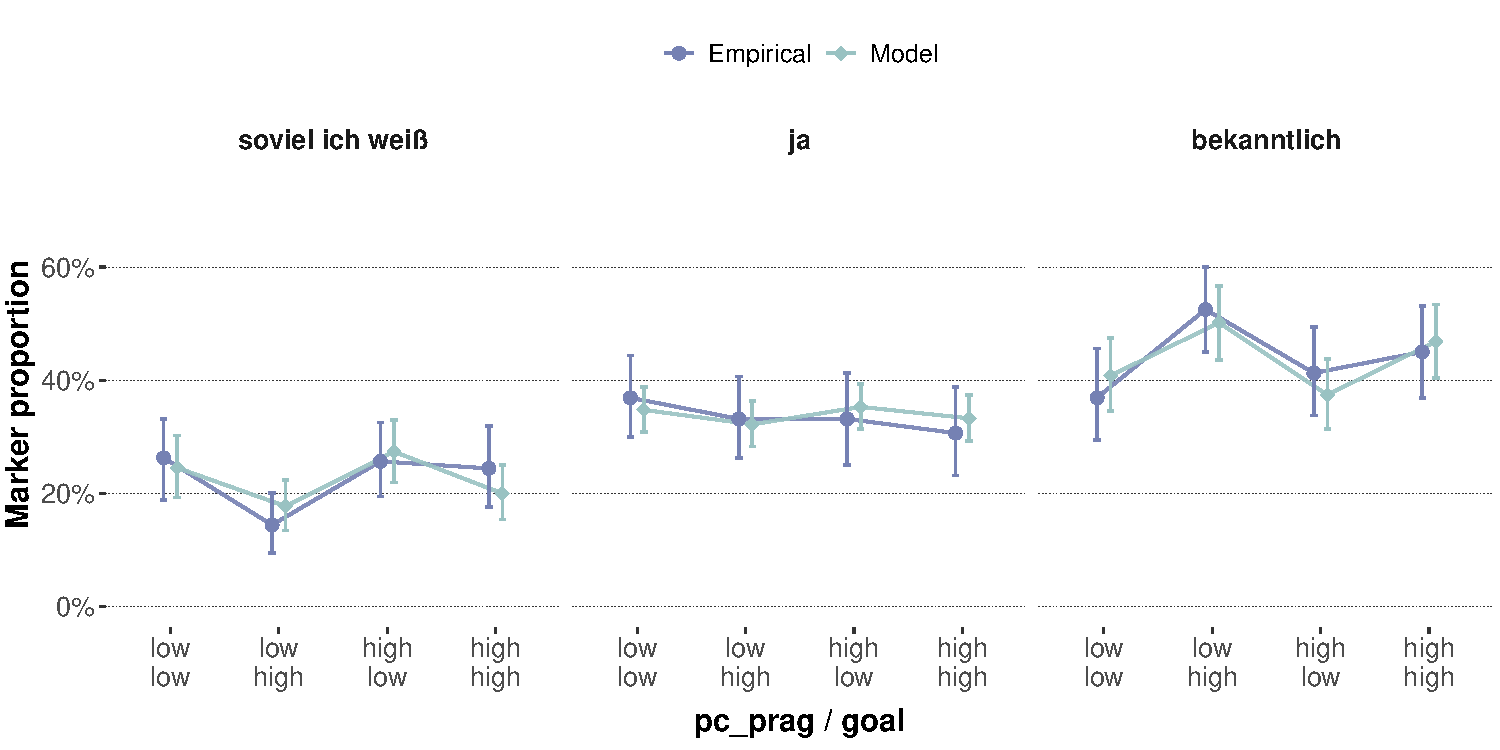
\includegraphics[width=\textwidth]{../../analysis/production_exp/plots/fig17c_facet_by_marker.pdf}
    \caption{Production experiment ($N\!=\!80$): lower controversy and higher speaker goal strength favour stricter-threshold markers.}\label{fig:production}
  \end{subfigure}\hfill
  \begin{subfigure}[b]{0.49\textwidth}
    \centering
    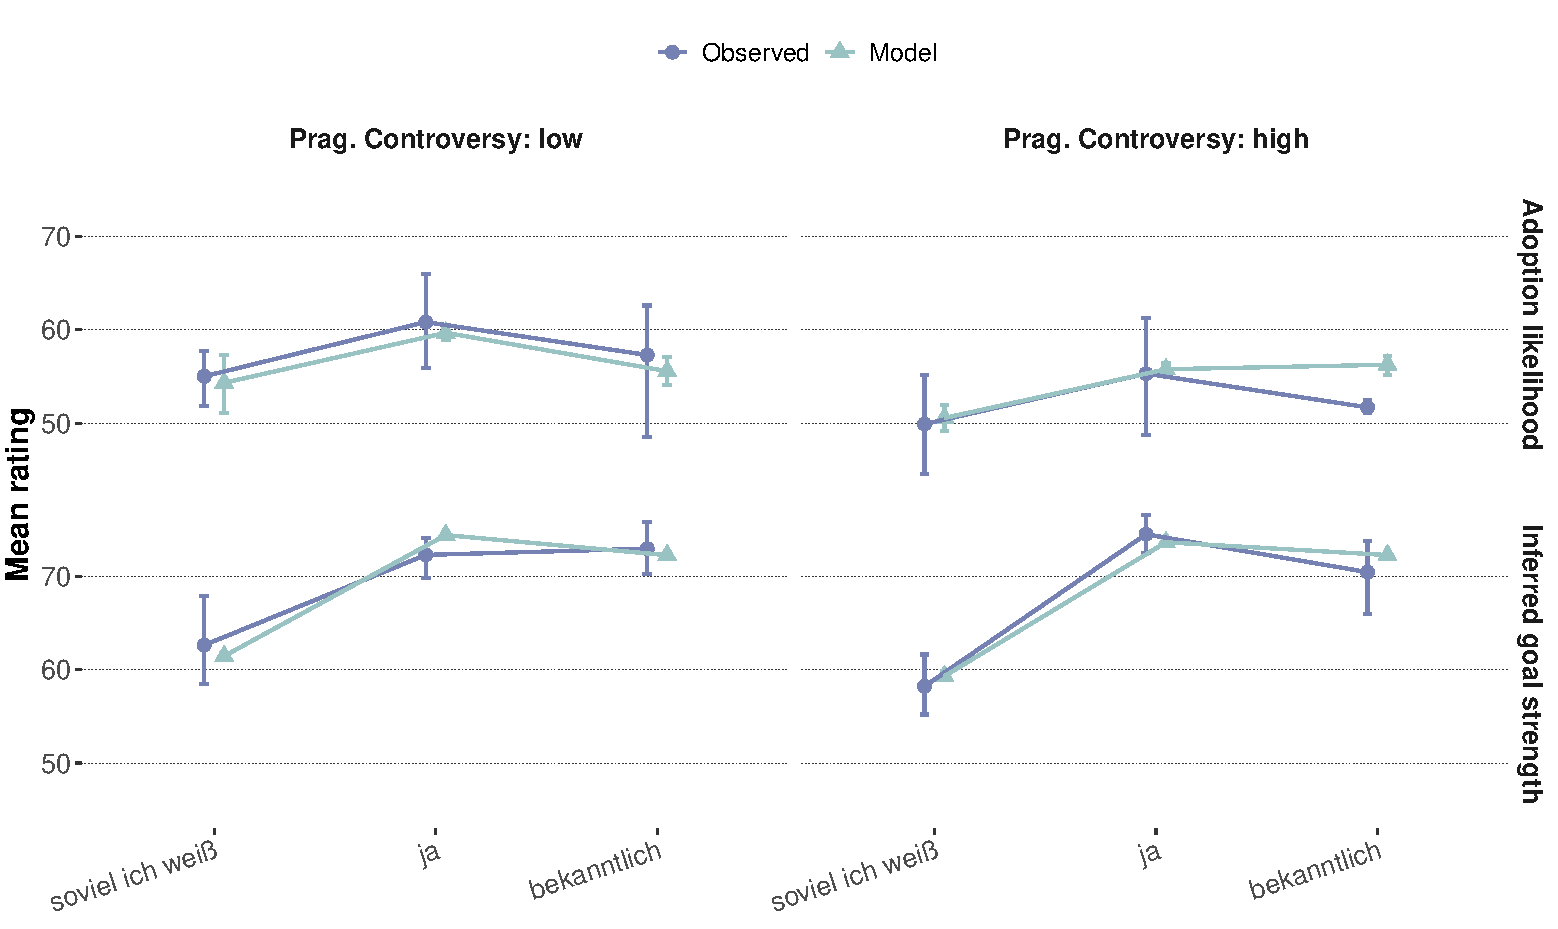
\includegraphics[width=\textwidth]{../../analysis/comprehension_exp/plots/fig7_rsa_base_vs_enhanced.pdf}
    \caption{Comprehension experiment ($N\!=\!80$): stricter-threshold markers increase inferred goal strength, while adoption reveals discounting when contextual support is low.}\label{fig:comprehension}
  \end{subfigure}

  \caption{Model and experimental results.
  Points show means; error bars show bootstrap 95\% confidence intervals.}
  \label{fig:all-results}
\end{figure}
\clearpage
\begin{figure}[h!]
  \centering
  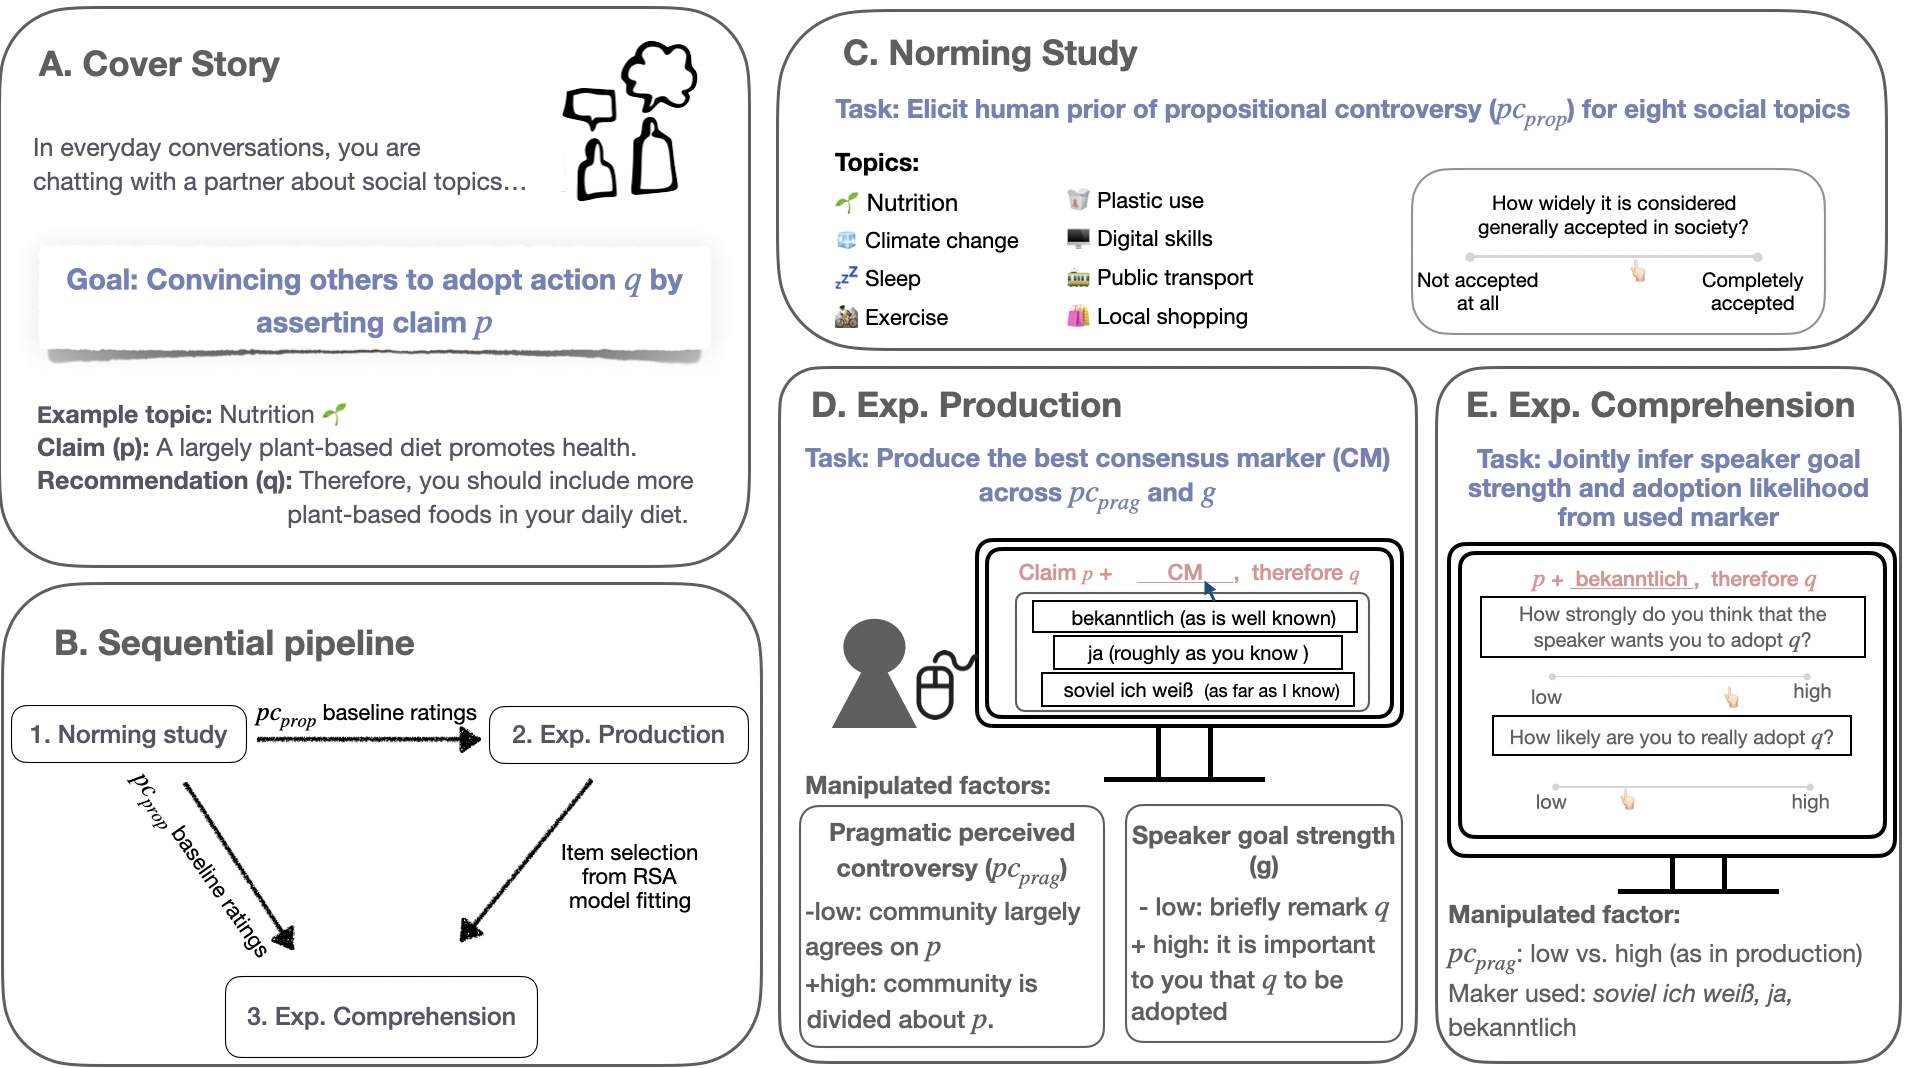
\includegraphics[width=\textwidth]{overview.png}
  \caption{Experimental pipeline.
  (A)~Participants discuss social topics with a partner, with $p$ serving as support for a recommendation $q$.
  (B)~Sequential design: a norming study establishes baseline propositional controversy, followed by production and comprehension experiments.
  (C)~Norming: eight topics rated for propositional controversy.
  (D)~Production: participants select the best consensus marker given manipulated pragmatic controversy and goal strength.
  (E)~Comprehension: participants infer speaker goal strength and adoption likelihood from marker-containing utterances.}
  \label{fig:overview}
\end{figure}

\textbf{References:}
\renewcommand{\bibsection}{}
\setlength{\bibsep}{0pt}
\setlength{\columnsep}{10pt}
{\footnotesize
\begin{multicols}{2}
\bibliographystyle{unsrtnat}
\bibliography{references}
\end{multicols}
}
\end{document}
